\kommentar{Zweitore}

\begin{karte}{Worum handelt sich bei einem Zweitor?}
	Ein Zweitor ist ein Vierpol bei welchem immer zwei als Paar auftreten. Die Spannungen und Ströme sind wie im Schema eingezeichnet definiert. Es muss immer auf das Vorzeichen geachtet werden. Ansonsten funktionieren die gesamten Rechenregeln nicht.
	
	\centering{\scalebox{.9}{%Autor: Simon Walker
%Version: 1.0
%Datum: 25.06.2020
%Lizenz: CC BY-NC-SA


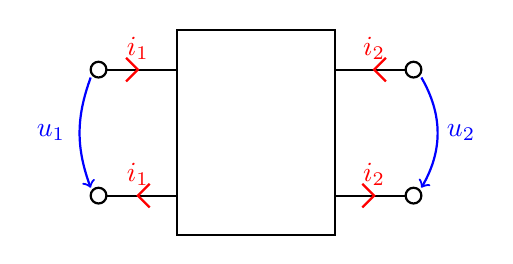
\begin{tikzpicture}

%Symbol
\draw[thick] (-1, -1.3) rectangle (1, 1.3);
\draw[thick] (-1,0.8) -- (-2,0.8);
\draw[thick, fill=white] (-2,0.8) circle (0.1);
\draw[thick] (-1,-0.8) -- (-2,-0.8);
\draw[thick, fill=white] (-2,-0.8) circle (0.1);

\draw[thick] (1,0.8) -- (2,0.8);
\draw[thick, fill=white] (2,0.8) circle (0.1);
\draw[thick] (1,-0.8) -- (2,-0.8);
\draw[thick, fill=white] (2,-0.8) circle (0.1);

%Strompfeile
\draw[red, thick] (-1.5, 0.8) node[above, red] {$i_1$} ++(-0.15, 0.15) -- ++(0.15, -0.15) -- ++(-0.15, -0.15);
\draw[red, thick] (-1.5, -0.8) node[above, red] {$i_1$} ++(0.15, 0.15) -- ++(-0.15, -0.15) -- ++(0.15, -0.15);

\draw[red, thick] (1.5, 0.8) node[above, red] {$i_2$} ++(0.15, 0.15) -- ++(-0.15, -0.15) -- ++(0.15, -0.15);
\draw[red, thick] (1.5, -0.8) node[above, red] {$i_2$} ++(-0.15, 0.15) -- ++(0.15, -0.15) -- ++(-0.15, -0.15);

%Spannungspfeile
\draw[blue, ->, thick, out=-110, in=110] (-2.1, 0.7) to (-2.1, -0.7);
\node[left, blue] at (-2.3,0){$u_1$};

\draw[blue, ->, thick, out=-60, in=60] (2.1, 0.7) to (2.1, -0.7);
\node[right, blue] at (2.3,0){$u_2$};


\end{tikzpicture}
}}	
\end{karte}

\begin{karte}{Was versteht man im Bezug auf Zweitore unter Passivität, Reziprozität und Symmetrie?}
	\textbf{Passivität:} Die Leistung die das Zweitor aufnimmt ist grösser als 0 ($P\ge 0$)\\
	\textbf{Reziprozität:} Ist die Symmetrie bezüglich dem Ausgang. Die Ströme durch die Amperemeter (blau umkreist) müssen gleich sein.\\
	\textbf{Symmetrie:} Die Ströme durch die Quelle (grün umkreist) müssen ebenfalls gleich sein.
	
	\centering{\scalebox{.7}{%Autor: Simon Walker
%Version: 1.0
%Datum: 25.06.2020
%Lizenz: CC BY-NC-SA


\begin{circuitikz}
%Symbol1
\draw[thick] (-1, -0.8) rectangle (1, 0.8);
\draw (-1, 0.5) to[short, -o] (-2, 0.5);
%\draw[thick] (-1,0.5) -- (-2,0.5);
%\draw[thick, fill=white] (-2,0.5) circle (0.1);
\draw (-1, -0.5) to[short, -o] (-2, -0.5);
%\draw[thick] (-1,-0.5) -- (-2,-0.5);
%\draw[thick, fill=white] (-2,-0.5) circle (0.1);

\draw[thick] (1,0.5) -- (2,0.5);
\draw[thick, fill=white] (2,0.5) circle (0.1);
\draw[thick] (1,-0.5) -- (2,-0.5);
\draw[thick, fill=white] (2,-0.5) circle (0.1);

%Strompfeile
\draw[red, thick] (-1.5, 0.5) node[above, red] {$i_1$} ++(-0.15, 0.15) -- ++(0.15, -0.15) -- ++(-0.15, -0.15);

\draw[red, thick] (1.5, 0.5) node[above, red] {$i_2$} ++(0.15, 0.15) -- ++(-0.15, -0.15) -- ++(0.15, -0.15);

%Quelle
\draw (-2,0.5) to[short] (-2,1) to[short] (-2.5, 1)	to[american voltage source] (-2.5 ,-1) to[short] (-2,-1) to[short] (-2, -0.5);

%Amperemeter
\draw (2,0.5) to[short] (2,1) to[short] (2.5, 1) to node[draw,circle,fill=white] {A} (2.5 ,-1) to[short] (2,-1) to[short] (2, -0.5);

%Einkreisen
\draw[green, very thick] (-1.5, 0.5) circle (0.5);
\draw[blue, very thick] (1.5, 0.5) circle (0.5);


\begin{scope}[shift={(7,0)}]
	%Symbol2
	\draw[thick] (-1, -0.8) rectangle (1, 0.8);
	\draw (-1, 0.5) to[short, -o] (-2, 0.5);
	%\draw[thick] (-1,0.5) -- (-2,0.5);
	%\draw[thick, fill=white] (-2,0.5) circle (0.1);
	\draw (-1, -0.5) to[short, -o] (-2, -0.5);
	%\draw[thick] (-1,-0.5) -- (-2,-0.5);
	%\draw[thick, fill=white] (-2,-0.5) circle (0.1);
	
	\draw[thick] (1,0.5) -- (2,0.5);
	\draw[thick, fill=white] (2,0.5) circle (0.1);
	\draw[thick] (1,-0.5) -- (2,-0.5);
	\draw[thick, fill=white] (2,-0.5) circle (0.1);
	
	%Strompfeile
	\draw[red, thick] (-1.5, 0.5) node[above, red] {$i_1$} ++(-0.15, 0.15) -- ++(0.15, -0.15) -- ++(-0.15, -0.15);
	
	\draw[red, thick] (1.5, 0.5) node[above, red] {$i_2$} ++(0.15, 0.15) -- ++(-0.15, -0.15) -- ++(0.15, -0.15);
	
	%Quelle
	\draw (-2,0.5) to[short] (-2,1) to[short] (-2.5, 1)	to node[draw,circle,fill=white] {A} (-2.5 ,-1) to[short] (-2,-1) to[short] (-2, -0.5);
	
	%Amperemeter
	\draw (2,0.5) to[short] (2,1) to[short] (2.5, 1) to[american voltage source] (2.5 ,-1) to[short] (2,-1) to[short] (2, -0.5);
	
	%Einkreisen
	\draw[green, very thick] (1.5, 0.5) circle (0.5);
	\draw[blue, very thick] (-1.5, 0.5) circle (0.5);
	
\end{scope}


\end{circuitikz}
}}
\end{karte}
